\documentclass[../main.tex, class=article, 12pt]{subfiles}
\usepackage{float}
\usepackage{amsthm}
\usepackage{amsmath}
\usepackage{amssymb}
\usepackage{hyperref}
\usepackage{caption}
\usepackage{mathtools}
\usepackage{graphicx}
\usepackage{todonotes}
\usepackage{tcolorbox}
\graphicspath{{./images}}




\begin{document}
Algebricamente possiamo considerare le le tralsazioni come somme e 
le dilatazione-contrazioni come moltiplicazioni. 


\subsection{traslazioni verticali}\label{sec:traslazioni_verticali}
dato un $ y_0 > 0 $ il grafico della funzione $ y =f(x) + y_0 $ si ottiene traslando
in alto di $ y_0 $ ed il grafico della funzione $ y = f(x) - y_0 $ si ottiene traslando
verso il basso di $ y_0 > 0 $.
\begin{figure}[H]
  	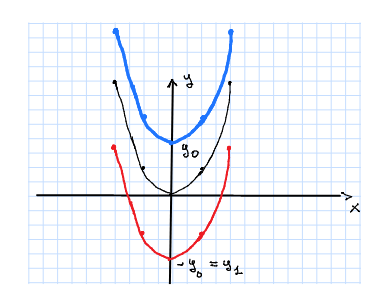
\includegraphics[width=\linewidth]{es_traslazione_verticale.png}
  	\caption{ROSSO: $ y = f(x) + y_0 $, BLU: $ f(x)-y_0 = f(x)+y_1 $}
        \label{fig:es_traslazione_verticale.png}
\end{figure}



\subsection{traslazioni orizzontali}\label{sec:traslazioni_orizzontali}
dato un $ x_0 > 0 $ il grafico della funzione $ y =f(x) + x_0 $ si ottiene traslando
in alto di $ x_0 $ ed il grafico della funzione $ y = f(x) - x_0 $ si ottiene traslando
verso il basso di $ x_0 > 0 $.
\begin{figure}[H]
  	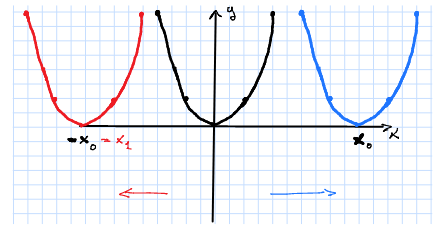
\includegraphics[width=\linewidth]{es_traslazione_orizzontale.png}
        \caption{ROSSO: $f(x+x_0) = f(x- x_1) $, BLU: $f(x-x_0)$} 
        \label{fig:es_traslazione_orizzontale.png}
\end{figure}



\subsection{dilatazioni e contrazioni verticali}\label{sec:dilatazioni_e_contrazioni_verticali}
dato un $ k > 1 $ il grafico della funzione $ y = f(x)/k$ si ottiene contraendo di $ a $ lungo 
l'asse $ y $ ed il grafico della funzione $ y = af(x)$ si ottiene dilatando di $ a $
lungo l'asse delle $ y $.


\begin{figure}[H]
  	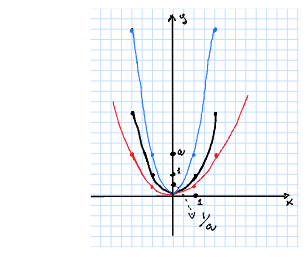
\includegraphics[width=\linewidth]{es_dilatazione_verticale.png}
  	\caption{}
        \label{fig:es_dilatazione_verticale.png}
\end{figure}




\subsection{dilatazioni e contrazioni orizzontali}\label{sec:dilatazioni_e_contrazioni_verticali}
dato un $ k > 1 $ il grafico della funzione $ y = f(x/k)$ si ottiene dilatandoi di $ a $ lungo 
l'asse $ x $ ed il grafico della funzione $ y = f(ax)$ si ottiene contraendo di $ a $
lungo l'asse delle $ x $.

\begin{figure}[H]
  	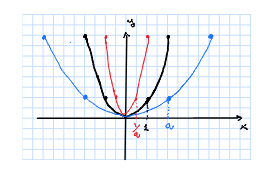
\includegraphics[width=\linewidth]{es_dilatazione_orizzontale.png}
  	\caption{}
        \label{fig:es_dilatazione_verticale.png}
\end{figure}



\subsection{Simmetrie}\label{sec:simmetrie}
\begin{definition}
        Una funzione $ f: A \to \mathbb{R} $ è detta:
        \begin{itemize}
                \item pari $ \forall  x \in A \Rightarrow -x \in A$ e $ f(-x) = f(x) $.
                \item dispari $ \forall  x \in A \Rightarrow -x \in A$ e $ f(-x) = -f(x) $.
        \end{itemize}
\end{definition}





\end{document}
